\documentclass[twoside]{book}

% Packages required by doxygen
\usepackage{fixltx2e}
\usepackage{calc}
\usepackage{doxygen}
\usepackage[export]{adjustbox} % also loads graphicx
\usepackage{graphicx}
\usepackage[utf8]{inputenc}
\usepackage{makeidx}
\usepackage{multicol}
\usepackage{multirow}
\PassOptionsToPackage{warn}{textcomp}
\usepackage{textcomp}
\usepackage[nointegrals]{wasysym}
\usepackage[table]{xcolor}

% Font selection
\usepackage[T1]{fontenc}
\usepackage[scaled=.90]{helvet}
\usepackage{courier}
\usepackage{amssymb}
\usepackage{sectsty}
\renewcommand{\familydefault}{\sfdefault}
\allsectionsfont{%
  \fontseries{bc}\selectfont%
  \color{darkgray}%
}
\renewcommand{\DoxyLabelFont}{%
  \fontseries{bc}\selectfont%
  \color{darkgray}%
}
\newcommand{\+}{\discretionary{\mbox{\scriptsize$\hookleftarrow$}}{}{}}

% Page & text layout
\usepackage{geometry}
\geometry{%
  a4paper,%
  top=2.5cm,%
  bottom=2.5cm,%
  left=2.5cm,%
  right=2.5cm%
}
\tolerance=750
\hfuzz=15pt
\hbadness=750
\setlength{\emergencystretch}{15pt}
\setlength{\parindent}{0cm}
\setlength{\parskip}{3ex plus 2ex minus 2ex}
\makeatletter
\renewcommand{\paragraph}{%
  \@startsection{paragraph}{4}{0ex}{-1.0ex}{1.0ex}{%
    \normalfont\normalsize\bfseries\SS@parafont%
  }%
}
\renewcommand{\subparagraph}{%
  \@startsection{subparagraph}{5}{0ex}{-1.0ex}{1.0ex}{%
    \normalfont\normalsize\bfseries\SS@subparafont%
  }%
}
\makeatother

% Headers & footers
\usepackage{fancyhdr}
\pagestyle{fancyplain}
\fancyhead[LE]{\fancyplain{}{\bfseries\thepage}}
\fancyhead[CE]{\fancyplain{}{}}
\fancyhead[RE]{\fancyplain{}{\bfseries\leftmark}}
\fancyhead[LO]{\fancyplain{}{\bfseries\rightmark}}
\fancyhead[CO]{\fancyplain{}{}}
\fancyhead[RO]{\fancyplain{}{\bfseries\thepage}}
\fancyfoot[LE]{\fancyplain{}{}}
\fancyfoot[CE]{\fancyplain{}{}}
\fancyfoot[RE]{\fancyplain{}{\bfseries\scriptsize Generated by Doxygen }}
\fancyfoot[LO]{\fancyplain{}{\bfseries\scriptsize Generated by Doxygen }}
\fancyfoot[CO]{\fancyplain{}{}}
\fancyfoot[RO]{\fancyplain{}{}}
\renewcommand{\footrulewidth}{0.4pt}
\renewcommand{\chaptermark}[1]{%
  \markboth{#1}{}%
}
\renewcommand{\sectionmark}[1]{%
  \markright{\thesection\ #1}%
}

% Indices & bibliography
\usepackage{natbib}
\usepackage[titles]{tocloft}
\setcounter{tocdepth}{3}
\setcounter{secnumdepth}{5}
\makeindex

% Hyperlinks (required, but should be loaded last)
\usepackage{ifpdf}
\ifpdf
  \usepackage[pdftex,pagebackref=true]{hyperref}
\else
  \usepackage[ps2pdf,pagebackref=true]{hyperref}
\fi
\hypersetup{%
  colorlinks=true,%
  linkcolor=blue,%
  citecolor=blue,%
  unicode%
}

% Custom commands
\newcommand{\clearemptydoublepage}{%
  \newpage{\pagestyle{empty}\cleardoublepage}%
}

\usepackage{caption}
\captionsetup{labelsep=space,justification=centering,font={bf},singlelinecheck=off,skip=4pt,position=top}

%===== C O N T E N T S =====

\begin{document}

% Titlepage & ToC
\hypersetup{pageanchor=false,
             bookmarksnumbered=true,
             pdfencoding=unicode
            }
\pagenumbering{roman}
\begin{titlepage}
\vspace*{7cm}
\begin{center}%
{\Large Sliding Puzzle \\[1ex]\large 1.\+0.\+0 }\\
\vspace*{1cm}
{\large Generated by Doxygen 1.8.11}\\
\end{center}
\end{titlepage}
\clearemptydoublepage
\tableofcontents
\clearemptydoublepage
\pagenumbering{arabic}
\hypersetup{pageanchor=true}

%--- Begin generated contents ---
\chapter{File Index}
\section{File List}
Here is a list of all documented files with brief descriptions\+:\begin{DoxyCompactList}
\item\contentsline{section}{{\bfseries conio.\+h} }{\pageref{conio_8h}}{}
\item\contentsline{section}{\hyperlink{main_8c}{main.\+c} \\*The time class represents a moment of time }{\pageref{main_8c}}{}
\end{DoxyCompactList}

\chapter{File Documentation}
\hypertarget{main_8c}{}\section{main.\+c File Reference}
\label{main_8c}\index{main.\+c@{main.\+c}}


The time class represents a moment of time.  


{\ttfamily \#include $<$stdio.\+h$>$}\\*
{\ttfamily \#include $<$stdlib.\+h$>$}\\*
{\ttfamily \#include $<$time.\+h$>$}\\*
{\ttfamily \#include $<$stdbool.\+h$>$}\\*
{\ttfamily \#include $<$math.\+h$>$}\\*
Include dependency graph for main.\+c\+:
\nopagebreak
\begin{figure}[H]
\begin{center}
\leavevmode
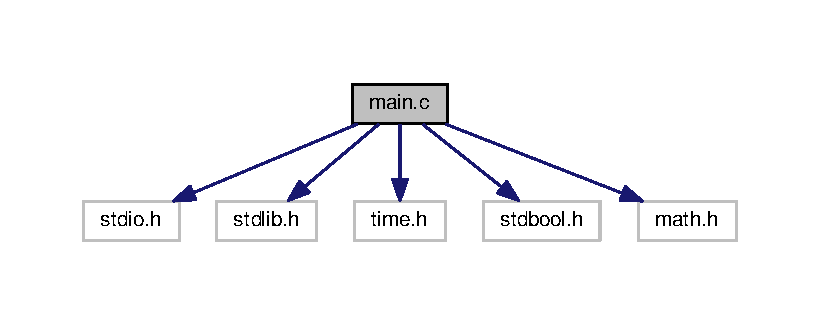
\includegraphics[width=350pt]{main_8c__incl}
\end{center}
\end{figure}
\subsection*{Macros}
\begin{DoxyCompactItemize}
\item 
\#define {\bfseries M\+AX}~4\hypertarget{main_8c_a392fb874e547e582e9c66a08a1f23326}{}\label{main_8c_a392fb874e547e582e9c66a08a1f23326}

\end{DoxyCompactItemize}
\subsection*{Functions}
\begin{DoxyCompactItemize}
\item 
void \hyperlink{main_8c_a4a6b044f2527429e874b0f20ff124293}{initialize\+Puzzle} ()
\item 
bool \hyperlink{main_8c_af7f1eb3ef4c37f02fd2805b165d93202}{check\+Puzzle} ()
\item 
void \hyperlink{main_8c_a82f678c1b45a0d174fbc628df09ce1ae}{print\+Puzzle} ()
\item 
void \hyperlink{main_8c_af37135a4231d56dd381f07e4a2552143}{control\+Puzzle} ()
\item 
int \hyperlink{main_8c_ae66f6b31b5ad750f1fe042a706a4e3d4}{main} ()
\end{DoxyCompactItemize}
\subsection*{Variables}
\begin{DoxyCompactItemize}
\item 
unsigned int {\bfseries coord\+\_\+x} = 0\hypertarget{main_8c_a1c378302ab218d0f8381d9edd5d05183}{}\label{main_8c_a1c378302ab218d0f8381d9edd5d05183}

\item 
unsigned int {\bfseries coord\+\_\+y} = 0\hypertarget{main_8c_ac4893a796d9fbe63eb53afddc95df8a8}{}\label{main_8c_ac4893a796d9fbe63eb53afddc95df8a8}

\item 
int {\bfseries sliding\+Puzzle} \mbox{[}M\+AX\mbox{]}\mbox{[}M\+AX\mbox{]}\hypertarget{main_8c_a3ec4a73b0230096b3f9b78ef3a20e2f2}{}\label{main_8c_a3ec4a73b0230096b3f9b78ef3a20e2f2}

\item 
bool {\bfseries is\+Existed} \mbox{[}16\mbox{]} = \{ false, \}\hypertarget{main_8c_abb3f762ab34f9c161d136e575d2127de}{}\label{main_8c_abb3f762ab34f9c161d136e575d2127de}

\item 
bool {\bfseries is\+Selected} = false\hypertarget{main_8c_aa878fd61855f549b463ca8e9ac7ad0f6}{}\label{main_8c_aa878fd61855f549b463ca8e9ac7ad0f6}

\end{DoxyCompactItemize}


\subsection{Detailed Description}
The time class represents a moment of time. 

\begin{DoxyAuthor}{Author}
Seulgi Kim \href{mailto:sgkim5955@gmail.com}{\tt sgkim5955@gmail.\+com} 
\end{DoxyAuthor}
\begin{DoxyDate}{Date}
2017/6/22 
\end{DoxyDate}
\begin{DoxyVersion}{Version}
1.\+0 
\end{DoxyVersion}
\hypertarget{main_8c_LICENSE}{}\subsection{L\+I\+C\+E\+N\+SE}\label{main_8c_LICENSE}
This program is free software, anybody can redistribute freely. 

\subsection{Function Documentation}
\index{main.\+c@{main.\+c}!check\+Puzzle@{check\+Puzzle}}
\index{check\+Puzzle@{check\+Puzzle}!main.\+c@{main.\+c}}
\subsubsection[{\texorpdfstring{check\+Puzzle()}{checkPuzzle()}}]{\setlength{\rightskip}{0pt plus 5cm}bool check\+Puzzle (
\begin{DoxyParamCaption}
{}
\end{DoxyParamCaption}
)}\hypertarget{main_8c_af7f1eb3ef4c37f02fd2805b165d93202}{}\label{main_8c_af7f1eb3ef4c37f02fd2805b165d93202}
Check if the puzzle board is completed. If numbers are assending ordered, board is completed and return true. Unless, board isn\textquotesingle{}t completed and return false, then continue game. \index{main.\+c@{main.\+c}!control\+Puzzle@{control\+Puzzle}}
\index{control\+Puzzle@{control\+Puzzle}!main.\+c@{main.\+c}}
\subsubsection[{\texorpdfstring{control\+Puzzle()}{controlPuzzle()}}]{\setlength{\rightskip}{0pt plus 5cm}void control\+Puzzle (
\begin{DoxyParamCaption}
{}
\end{DoxyParamCaption}
)}\hypertarget{main_8c_af37135a4231d56dd381f07e4a2552143}{}\label{main_8c_af37135a4231d56dd381f07e4a2552143}
Check which piece of puzzle is next to blank(\#). And if user inputs puzzle number, change current puzzle board using swap. \index{main.\+c@{main.\+c}!initialize\+Puzzle@{initialize\+Puzzle}}
\index{initialize\+Puzzle@{initialize\+Puzzle}!main.\+c@{main.\+c}}
\subsubsection[{\texorpdfstring{initialize\+Puzzle()}{initializePuzzle()}}]{\setlength{\rightskip}{0pt plus 5cm}void initialize\+Puzzle (
\begin{DoxyParamCaption}
{}
\end{DoxyParamCaption}
)}\hypertarget{main_8c_a4a6b044f2527429e874b0f20ff124293}{}\label{main_8c_a4a6b044f2527429e874b0f20ff124293}
Initailize 4$\ast$4 puzzle board using random function. There isn\textquotesingle{}t no duplicated number and numbers from 1 to 15. \index{main.\+c@{main.\+c}!main@{main}}
\index{main@{main}!main.\+c@{main.\+c}}
\subsubsection[{\texorpdfstring{main()}{main()}}]{\setlength{\rightskip}{0pt plus 5cm}int main (
\begin{DoxyParamCaption}
{}
\end{DoxyParamCaption}
)}\hypertarget{main_8c_ae66f6b31b5ad750f1fe042a706a4e3d4}{}\label{main_8c_ae66f6b31b5ad750f1fe042a706a4e3d4}
This is main function of sliding\+Puzzle \index{main.\+c@{main.\+c}!print\+Puzzle@{print\+Puzzle}}
\index{print\+Puzzle@{print\+Puzzle}!main.\+c@{main.\+c}}
\subsubsection[{\texorpdfstring{print\+Puzzle()}{printPuzzle()}}]{\setlength{\rightskip}{0pt plus 5cm}void print\+Puzzle (
\begin{DoxyParamCaption}
{}
\end{DoxyParamCaption}
)}\hypertarget{main_8c_a82f678c1b45a0d174fbc628df09ce1ae}{}\label{main_8c_a82f678c1b45a0d174fbc628df09ce1ae}
Print out current puzzle board. 
%--- End generated contents ---

% Index
\backmatter
\newpage
\phantomsection
\clearemptydoublepage
\addcontentsline{toc}{chapter}{Index}
\printindex

\end{document}
